\documentclass{article}
\usepackage{graphicx}
\begin{document}
\section*{Adding noise to data}
In fields like time series analysis or machine learning, it's often useful
to generate artificial datasets for testing code rather than go through the 
trouble of finding a dataset that meets some specifications. \newline \\0
Write a function that adds noise to otherwise `smooth' data. For instance, here's
a smooth function and the accompanying `noisy' version:
\begin{figure}[h]
\begin{center}
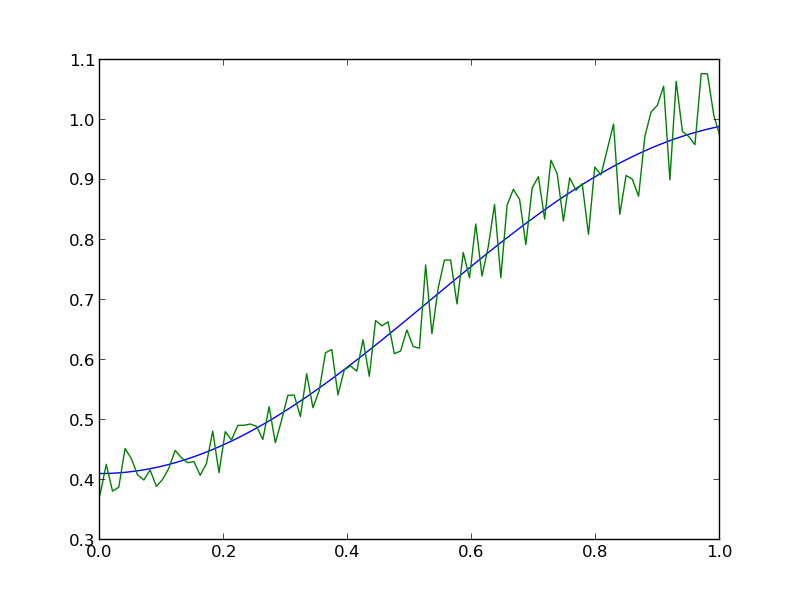
\includegraphics[height=150pt]{../pictures/noise.png}
\caption{$ y = sin(exp(cos(x))) $}
\end{center}
\end{figure}

This data is a good candidate for evaluating the performance of, say, a curve 
fitting function.
\end{document}
